\documentclass[slovene,11pt,a4paper]{article}
\usepackage[margin=2cm,bottom=2cm,foot=1.5cm]{geometry}
% \documentclass[slovene,11pt,a4paper]{article}
% \usepackage[margin=1.7cm,bottom=3cm,foot=1.5cm]{geometry}
\setlength{\parindent}{0pt}
\setlength{\parskip}{0.5ex}

\usepackage[pdftex]{graphicx}
\usepackage{pgffor}
\usepackage{subcaption}
% \usepackage{a4wide} %najaci package
\usepackage[utf8]{inputenc}
\usepackage[slovene]{babel}
\usepackage{color}
\usepackage{graphicx}
% \usepackage{subfigure}
\usepackage{imakeidx}
\usepackage{adjustbox}
\usepackage{float}
\usepackage{amsmath}
\usepackage{mathtools}
\usepackage{tikz}
\usepackage{amssymb}
\usepackage{listings}
\usepackage{siunitx}
\usepackage{hyperref}
\usepackage{amsfonts}
\usepackage{mathrsfs}

\def\phi{\varphi}
\def\eps{\varepsilon}
\def\theta{\vartheta}
\def\phi{\varphi}
\def\eps{\varepsilon}
\def\theta{\vartheta}

\newcommand{\thisyear}{2024/25}

\renewcommand{\Re}{\mathop{\rm Re}\nolimits}
\renewcommand{\Im}{\mathop{\rm Im}\nolimits}
\newcommand{\Tr}{\mathop{\rm Tr}\nolimits}
\newcommand{\diag}{\mathop{\rm diag}\nolimits}
\newcommand{\dd}{\,\mathrm{d}}
\newcommand{\ddd}{\mathrm{d}}
\newcommand{\ii}{\mathrm{i}}
\newcommand{\lag}{\mathcal{L}\!}
\newcommand{\ham}{\mathcal{H}\!}
\newcommand{\four}[1]{\mathcal{F}\!\left(#1\right)}
\newcommand{\bigO}[1]{\mathcal{O}\!\left(#1\right)}
\newcommand{\sh}{\mathop{\rm sinh}\nolimits}
\newcommand{\ch}{\mathop{\rm cosh}\nolimits}
\renewcommand{\th}{\mathop{\rm tanh}\nolimits}
\newcommand{\erf}{\mathop{\rm erf}\nolimits}
\newcommand{\erfc}{\mathop{\rm erfc}\nolimits}
\newcommand{\sinc}{\mathop{\rm sinc}\nolimits}
\newcommand{\rect}{\mathop{\rm rect}\nolimits}
\newcommand{\ee}[1]{\cdot 10^{#1}}
\newcommand{\inv}[1]{\left(#1\right)^{-1}}
\newcommand{\invf}[1]{\frac{1}{#1}}
\newcommand{\sqr}[1]{\left(#1\right)^2}
\newcommand{\half}{\frac{1}{2}}
\newcommand{\thalf}{\tfrac{1}{2}}
\newcommand{\pd}{\partial}
\newcommand{\Dd}[3][{}]{\frac{\ddd^{#1} #2}{\ddd #3^{#1}}}
\newcommand{\Pd}[3][{}]{\frac{\pd^{#1} #2}{\pd #3^{#1}}}
\newcommand{\avg}[1]{\left\langle#1\right\rangle}
\newcommand{\norm}[1]{\left\Vert #1 \right\Vert}
\newcommand{\braket}[2]{\left\langle #1 \vert#2 \right\rangle}
\newcommand{\obraket}[3]{\left\langle #1 \vert #2 \vert #3 \right \rangle}
\newcommand{\hex}[1]{\texttt{0x#1}}

\renewcommand{\iint}{\mathop{\int\mkern-13mu\int}}
\renewcommand{\iiint}{\mathop{\int\mkern-13mu\int\mkern-13mu\int}}
\newcommand{\oiint}{\mathop{{\int\mkern-15mu\int}\mkern-21mu\raisebox{0.3ex}{$\bigcirc$}}}

\newcommand{\wunderbrace}[2]{\vphantom{#1}\smash{\underbrace{#1}_{#2}}}

\renewcommand{\vec}[1]{\overset{\smash{\hbox{\raise -0.42ex\hbox{$\scriptscriptstyle\rightharpoonup$}}}}{#1}}
\newcommand{\bec}[1]{\mathbf{#1}}


\newcommand{\bi}[1]{\hbox{\boldmath{$#1$}}}
\newcommand{\bm}[1]{\hbox{\underline{$#1$}}}

\catcode`_=12
\begingroup\lccode`~=`_\lowercase{\endgroup\let~\sb}
\mathcode`_="8000

\title{
\sc\large Matematično-fizikalni praktikum \thisyear \\
\bigskip
\bf\Large 10.~naloga: Diferenčne metode za parcialne diferencialne enačbe
}
\author{Tadej Tomažič}
\date{}

\makeindex[columns=3, title=Alphabetical Index, intoc]

\begin{document}


\pagenumbering{gobble} 
\author{Tadej Tomažič}
\date{\today}

\maketitle

\newpage
\pagenumbering{arabic}
\tableofcontents
\listoffigures
\newpage
\vspace{-1cm}
\section{Navodilo}


Enorazsežna nestacionarna Sch\"odingerjeva enačba
\begin{equation*}
  \left(i\hbar\Pd{}{t}-H\right)\psi(x,t)=0
\end{equation*}
je osnovno orodje za nerelativistični opis časovnega razvoja kvantnih stanj v različnih potencialih. Tu obravnavamo samo od časa neodvisne hamiltonske operatorje
\begin{equation*}
  H=-\frac{\hbar^2}{2m}\Pd[2]{}{x}+V(x)\>.
\end{equation*}
Z menjavo spremenljivk $H/\hbar\mapsto H$, $x\sqrt{m/\hbar}\mapsto x$ in $V(x\sqrt{m/\hbar})/\hbar\mapsto V(x)$, efektivno postavimo $\hbar=m=1$,
\begin{equation}
  H=-\frac12\Pd[2]{}{x}+V(x)\>.
  \label{eq:hamilton}
\end{equation}


Razvoj stanja $\psi(x,t)$ v stanje $\psi(x,t+\Delta t)$ opišemo s približkom
\begin{equation}
  \psi(x,t+\Delta t)=e^{-\ii H \Delta t} \psi(x,t)\approx \frac{1-\thalf \ii H \Delta t}{1+\thalf \ii H \Delta t}\psi(x,t)\>,
  \label{eq:razvoj}
\end{equation}
ki je unitaren in je reda $\mathcal{O}(\Delta t^3)$. Območje $a\leq x\leq b$ diskretiziramo na krajevno mrežo $x_j=a+j\Delta x$ pri $0\leq j<N$, $\Delta x = (b-a)/(N-1)$, časovni razvoj pa spremljamo ob časih $t_n=n\Delta t$. Vrednosti valovne funkcije in potenciala v mrežnih točkah ob času $t_n$ označimo $\psi(x_j,t_n)=\psi_j^n$ oziroma $V(x_j)=V_j$. Krajevni odvod izrazimo z diferenco
\begin{equation*}
  \Psi''(x)\approx \frac{\psi(x+\Delta x,t)-2\psi(x,t)+\psi(x-\Delta x,t)}{\Delta x^2}=\frac{\psi_{j+1}^n - 2\psi_j^n+\psi_{j-1}^n}{\Delta x^2}\>.
\end{equation*}
Ko te približke vstavimo v enačbo (\ref{eq:razvoj}) in razpišemo Hamiltonov operator po enačbi (\ref{eq:hamilton}), dobimo sistem enačb
\begin{equation*}
  \psi_j^{n+1}-\ii\frac{\Delta t}{4\Delta x^2}\left[\psi_{j+1}^{n+1}-2\psi_j^{n+1}+\psi_{j-1}^{n+1}\right] + \ii\frac{\Delta t}{2}V_j \psi_j^{n+1}=  \psi_j^{n}+\ii\frac{\Delta t}{4\Delta x^2}\left[\psi_{j+1}^{n}-2\psi_j^{n}+\psi_{j-1}^{n}\right] - \ii\frac{\Delta t}{2}V_j \psi_j^{n}\>,
\end{equation*}
v notranjih točkah mreže, medtem ko na robu ($j\leq 0$ in $j\geq N$) postavimo $\psi_j^n=0$. Vrednosti valovne funkcije v točkah $x_j$ uredimo v vektor
\begin{equation*}
\boldsymbol{\Psi}^n=(\psi_1^n,\ldots,\psi_{N-1}^n)^T
\end{equation*}
in sistem prepišemo v matrično obliko
\begin{equation*}
  \mathsf{A}\boldsymbol{\Psi}^{n+1}=\mathsf{A}^\ast \boldsymbol{\Psi}^n,\qquad
  \mathsf{A}=\begin{pmatrix}
  d_1 & a \\
  a   & d_2 & a \\
  & a & d_3 & a \\
  & & \ddots & \ddots & \ddots \\
  & & & a & d_{N-2} & a \\
  & & & & a & d_{N-1}
  \end{pmatrix}\>,
\end{equation*}
kjer je
\begin{equation*}
  b=\ii \frac{\Delta t}{2 \Delta x^2},\qquad a=-\frac{b}{2},\qquad d_j = 1+b+\ii \frac{\Delta t}{2}V_j\>.
\end{equation*}
Dobili smo torej matrični sistem, ki ga moramo rešiti v vsakem časovnem koraku, da iz stanja $\boldsymbol{\Psi}^n$ dobimo stanje $\boldsymbol{\Psi}^{n+1}$. Matrika $\mathsf{A}$ in vektor $\boldsymbol{\Psi}$ imata kompleksne elemente, zato račun najlažje opraviš v kompleksni aritmetiki\footnote{
  {\tt \#include <complex.h>} v {\tt c}, {\tt \#include <complex>} v {\tt c++}, {\tt from cmath import *} za kompleksne funkcije v Pythonu (sama kompleksna aritmetika pa je vgrajena).
}. Izkaže se, da so za zadovoljivo natančnost višji redi nujni!

Z uporabljenim približkom za drugi odvod reda $\mathcal{O}(\Delta x^2)$ dobimo tridiagonalno matriko. Z diferencami višjih redov dobimio večdiagonalno (pasovno) matriko, a dosežemo tudi večjo krajevno natančnost. Diference višjih redov so bile predstavljene na predavanjih, lahko 
pa jih hitro izračunaš na primer v Mathematici s funkcijo
\begin{center}
  \tt FD[m_,n_,s_] := CoefficientList[Normal[Series[x\string^s Log[x]\string^m, \{x, 1, n\}]/h\string^m], x];
\end{center}
kjer je {\tt m} red diference (odvoda), {\tt n} število intervalov širine $h=\Delta x$, ki jih diferenca upošteva, in {\tt s} število intervalov med točko, kjer diferenco računamo, in skrajno levo točko diferenčne sheme. Zgornjo tritočkovno sheme za drugo diferenco dobimo kot {\tt FD[2, 2, 1]}, saj se razpenja čez {\tt n=2} intervala, sredinska točka pa je v točki z indeksom {\tt s=1}. 

Tudi korakanje v času je mogoče izboljšati z uporabo Pad\'ejeve aproksimacije za eksponentno funkcijo, glej \cite{dijk} in/ali predavanja. 


{\it Naloga\/}: Spremljaj časovni razvoj začetnega stanja
\begin{equation*}
  \Psi(x,0)=\sqrt{\frac{\alpha}{\sqrt{\pi}}} e^{-\alpha^2 (x-\lambda)^2/2}
\end{equation*}
v harmonskem potencialu $V(x)=\frac12 kx^2$, kjer je v naravnih enotah $\alpha=k^{1/4}$, $\omega=\sqrt{k}$. Analitična rešitev je koherentno stanje
\begin{equation*}
  \psi(x,t)=\sqrt{\frac{\alpha}{\sqrt{\pi}}} \exp\left[-\frac12 \left(\xi-\xi_\lambda \cos\omega t\right)^2 - \ii \left(\frac{\omega t}{2}+\xi\xi_\lambda \sin\omega t - \frac14 \xi_\lambda^2 \sin 2 \omega t\right)\right]\>,
\end{equation*}
kjer je $\xi=\alpha x$, $\xi_\lambda=\alpha \lambda$. Postavi parametre na $\omega=0.2$, $\lambda=10$. Krajevno mrežo vpni v interval $[a,b]=[-40,40]$ z $N=300$ aktivnimi točkami. Nihajni čas je $T=2\pi/\omega$ -- primerno prilagodi časovni korak $\Delta t$ in stanje opazuj deset period.

Opazuj še razvoj gaussovskega valovnega paketa
\begin{equation*}
  \psi(x,0)=(2\pi \sigma_0^2)^{-1/4} e^{\ii k_0(x-\lambda)}e^{-(x-\lambda)^2/(2\sigma_0)^2}
\end{equation*}
v prostoru brez potenciala. Postavi $\sigma_0=1/20$, $k_0=50\pi$, $\lambda=0.25$ in območje $[a,b]=[-0.5,1.5]$ ter $\Delta t=2\Delta x^2$. Časovni razvoj spremljaj, dokler težišče paketa ne pride do $x\approx 0.75$. Analitična rešitev je
\begin{equation*}
  \psi(x,t)=\frac{(2\pi \sigma_0^2)^{-1/4}}{\sqrt{1+\ii t/(2\sigma_0^2)}} \exp\left[
    \frac{-(x-\lambda)^2/(2\sigma_0)^2+\ii k_0(x-\lambda)-\ii k_0^2 t/2}{1+\ii t/(2\sigma_0^2)}
    \right]
\end{equation*}

V vseh obravnavanih primerih ugotovi in uporabi dovolj natančno metodo višjega reda.


\begin{thebibliography}{99}
\setlength{\itemsep}{.2\itemsep}\setlength{\parsep}{.5\parsep}
\bibitem{dijk} W. van Dijk, F. M. Toyama, Phys. Rev. E {\bf 75}, 036707 (2007).
\end{thebibliography}
\section{Rešitev}

Najprej si poglejmo avtokorelacijo za obe sovi.
\begin{figure}[h]
    \centering
    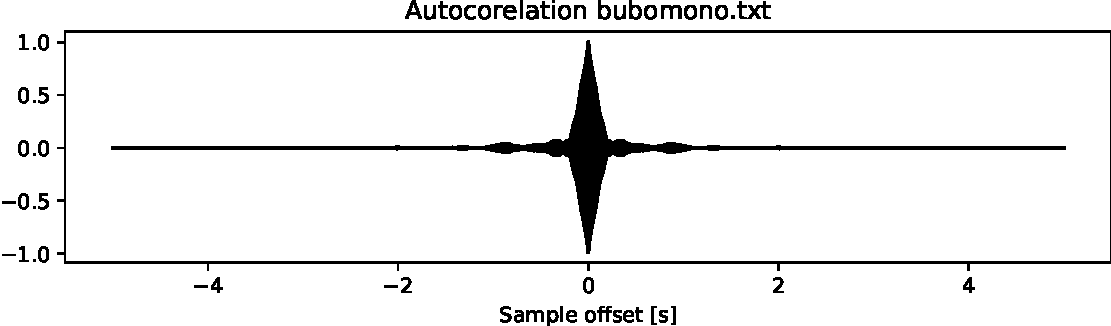
\includegraphics[width=12cm]{pdfs/bubomono.txt_acor.pdf}
    \vspace{10pt}
    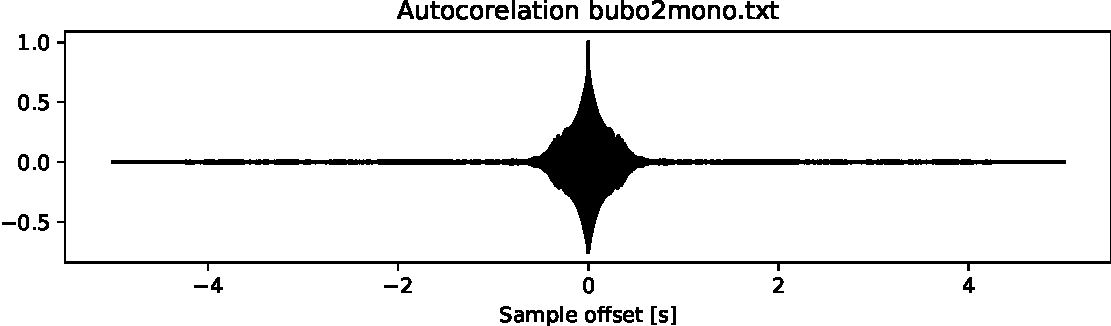
\includegraphics[width=12cm]{pdfs/bubo2mono.txt_acor.pdf}
    \caption{Avtokorelacija signala sov}
\end{figure}

Preden sem koreliral signal sem vektorja samplov normiral, tako da je
"najmočnejši" signal 1. To pomeni \[\|x\|_\infty = \max_i |x_i|\]

Poglejmo si še korelacije med sovami in posnetki:
\newpage
\begin{figure}[h]
    \centering
    \foreach \mix in {mix, mix1, mix2, mix22} {
        \foreach \sova in {bubomono, bubo2mono}{
            \includegraphics[width=8cm]{pdfs/cor_\mix.txt_\sova.txt.pdf}
        }
    }
    \caption{Korelacija sov in posnetkov iz narave}
\end{figure}
Tukaj je bila normalizacija drugače izbrana. Tukaj je bila narejena normalizacija korelacije. Če je varianca signala a $\sigma_a$,
potem je $ \mathbf{x} = \mathbf{x} / \left(\sigma_a \sigma_b |\mathbf{b}|\right)$. Sigma je izračunana z \verb|numpy.std()|.


Hitrosti so precej dolgčasno pričakovane ampak vseeno.
\begin{figure}[h]
    \centering
    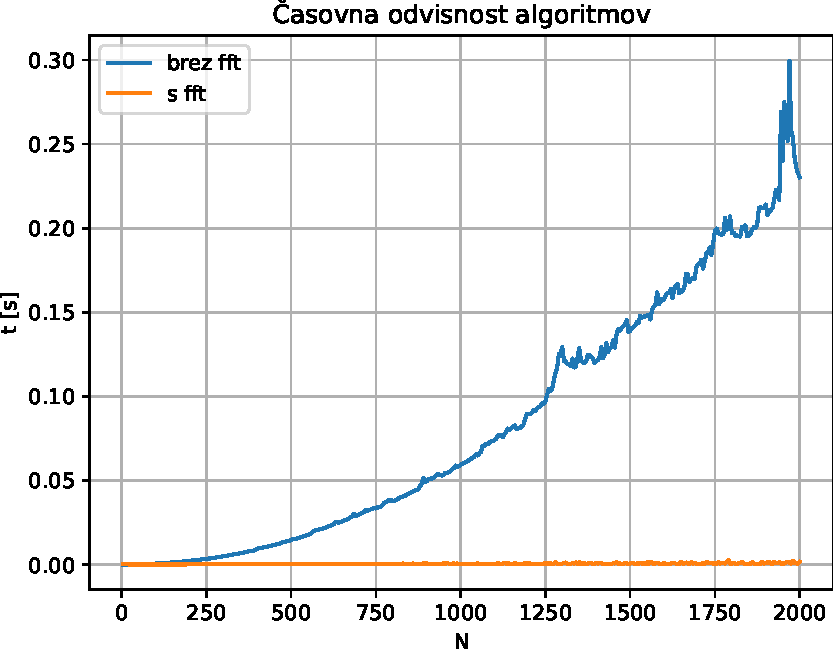
\includegraphics[width=8cm]{pdfs/cas-lin.pdf}
    \vspace{10pt}
    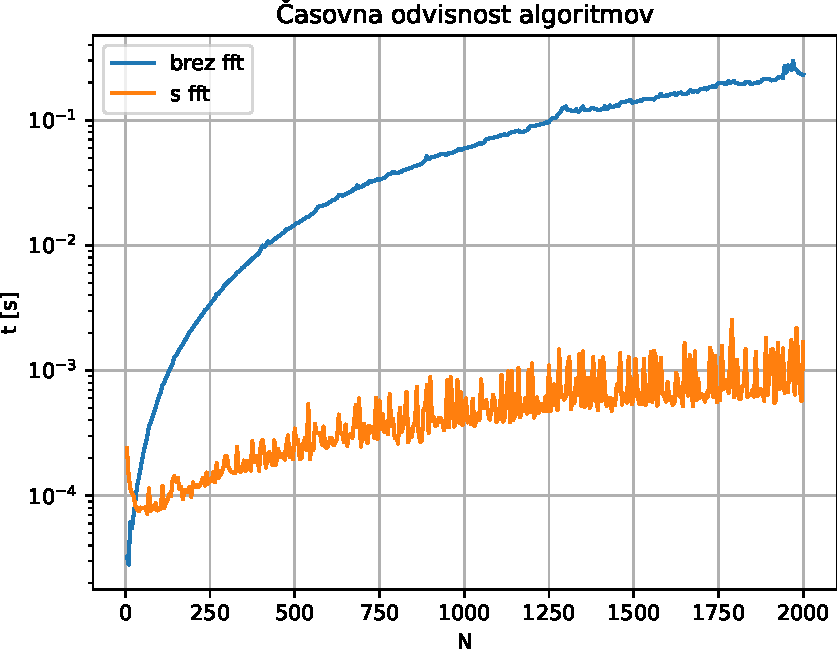
\includegraphics[width=8cm]{pdfs/cas-log.pdf}
    \caption{Hitrost algoritmov}
\end{figure}
\newpage
\section{Dodatna naloga}
Posnel sem dva človeka m in ž ko izgovarjata aaaaaaaaaaaa. Posnel sem jih tudi
ko bereta slovar. Gledal sem ali lahko spet zaznam ali gre za ž glas ali m glas.
Poglejmo si spektra njunega glasu.
\begin{figure}[h]
    \begin{center}
        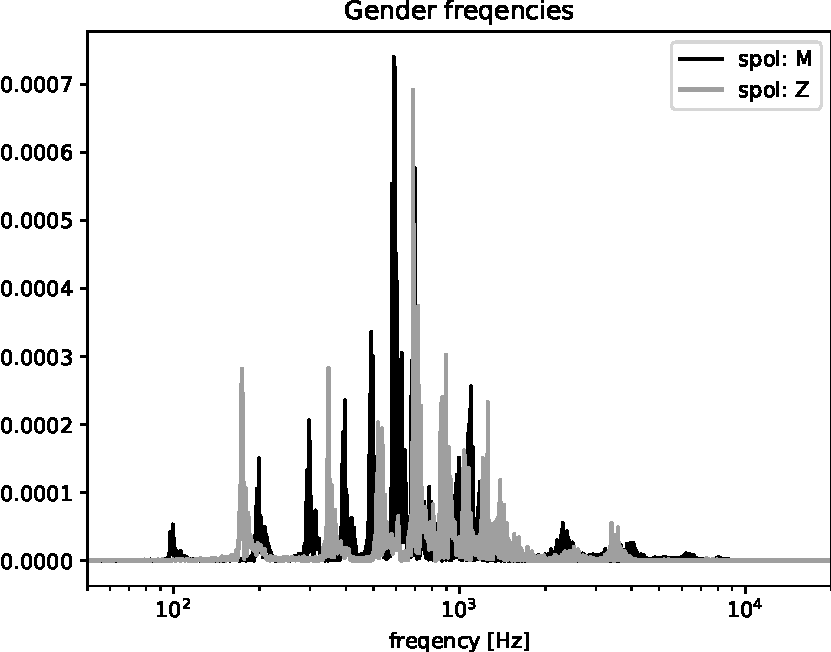
\includegraphics[width=12cm]{pdfs/fft_spol.pdf}
    \end{center}
    \caption{Barva glasu moškega in ženske}
\end{figure}

% Glasova sta bila prej normirana, saj je bil moški glas posnet bližje mikrofona.
% Poglejmo si zopet korelacijo med posnetki:
% \foreach \gender in {Z, M} {
%     \foreach \mix in {Glas\ 001, Glas\ 002}{
%         pdfs/cor_\gender_\mix.pdf 
%     }
% }
\begin{figure}[h]
    \begin{center}
        
    \foreach \gender in {Z, M} {%
        \foreach \mix in {001, 002} {%
            \includegraphics[width=8cm]{pdfs/cor_\gender_Glas\space\mix.pdf}%    
        }%
        \par
}%
    \end{center}
    
    \caption{Korelacija glasa človeka in posnetkov iz branja slovarja}
\end{figure}

\end{document}
